%Intro_Arduino_ComputerControl
\chapter{Introduction to the Arduino}

\objectives{
\item Explain how to use a prototyping board, including the identification of
which pins are electrically connected.
\item Demostrate proper soldering technique.
\item Describe the two primary functions included in every Arduino sketch, when
they are called, and what they do.
\item Compile and upload sketches to an Arduino.
\item Demonstrate the use of digital output on the Arduino by constructing 
several circuits involving blinking lights.
}

\review{
\item Voltage (electric potential).
\item Current.
\item Resistance.
\item Diodes and LEDs.
}

There are two ways in which we want our computers to communicate with our
physics experiments:
\begin{enumerate}
\item Have the computer control the experiment. For example, we could have the
computer turn on our apparatus, or turn it off. 
\item Have the experimental device provide data to the computer. The computer
can then record this data for later analysis.
\end{enumerate}
In both cases, we need something that goes between the
experimental measuring devices and the computer. These go-between pieces are
often called Data Acquisition (DAQ) boards. There are many different forms
of DAQs. They can cost anywhere from a few dollars to many thousands of
dollars.

In this lab, we will use a low cost DAQ, the plans for which the 
developers placed in the open-source world so that no one
would get royalties (including themselves) for the design (this is why the
boards are inexpensive). It is low cost, but not low
quality. The developers named their DAQ the ``Arduino''. There are many
different variations on the Arduino. We will specifically be using the
Arduino UNO.

Like all DAQs, the Arduino is fragile, so we will need to exercise some 
caution. Arduinos can be destroyed by putting too large a voltage or electrical 
current into the input pins. They also can be destroyed by mechanical means, 
such as being dropped or crushed.

By the end of this chapter, you will have successfully used an Arduino to 
communicate with an electric circuit. However, before we can interface with
a circuit, we have to build one.

%%%%%%%%%%%%%%%%%%%%%%%%%%%%%%%%%%%%%%%%%%%%%%%%%%%%%%%%%%%%%%%%%%%%%%%%%%%%%%%%

\section{Building circuits}

When you are first designing and constructing a circuit, you want to be able to 
easily and quickly make and revise electrical connections. Once the circuit
is designed, you often want to make it more permanent with solid connections
that cannot be jostled loose. We'll now consider how we go about building these
temporary and longer lasting circuits.

\subsection{Temporary circuits: the prototyping board}

Temporary circuits are usually built on a prototyping board, which is a plastic
board full of holes, as seen in Figure \ref{fig:protoboard_blank}. Each of the
holes in the prototyping board (sometimes a called a ``protoboard'' or 
``breadboard'') is a place where you can insert the lead from an electrical 
component, such as a resistor or capacitor, or a wire. 
(A ``lead'' is one of the wires
protruding from the component.)
\begin{figure}[hbp!]
\centering
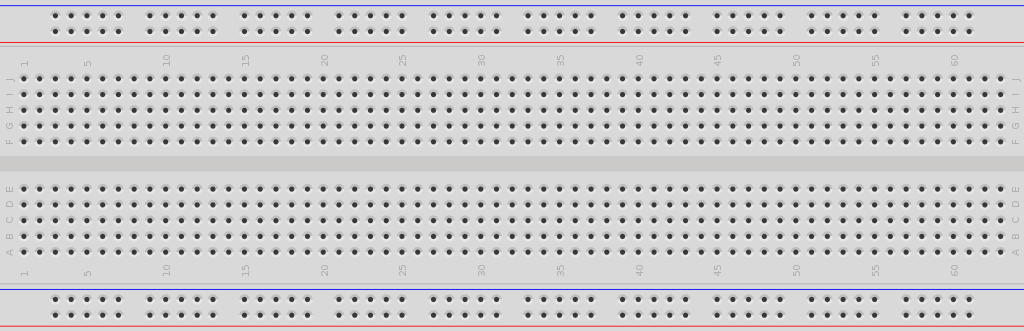
\includegraphics[width=0.8\textwidth]{protoboard_blank}
\caption[An empty prototyping board]{An empty prototyping board.}
\label{fig:protoboard_blank}
\end{figure}

The advantage of a prototyping board is that each of the holes is electrically 
connected to at least four other holes. Thus, by plugging leads wires 
into two connected holes, the leads or wires are now electrically 
connected to each other. The connections in a prototyping board are typically
as follows:
\begin{itemize}
\item All of the holes adjacent to each of the blue lines are connected. 
These are typically used for connections to an electrical ground or the
negative terminal of a power source.
\item All of the holes adjacent to each of the red lines are connected.
These are typically used for connections to an electrical power source 
(generally the positive terminal for DC power sources).
\item Each vertically oriented set of five holes in the center of the board
are connected.
\end{itemize}
These connections are illustrated in Figure \ref{fig:protoboard_connections}.
Please note that not all prototyping boards are alike, and the connections
may vary from board to board.
\begin{figure}[hbp!]
\centering
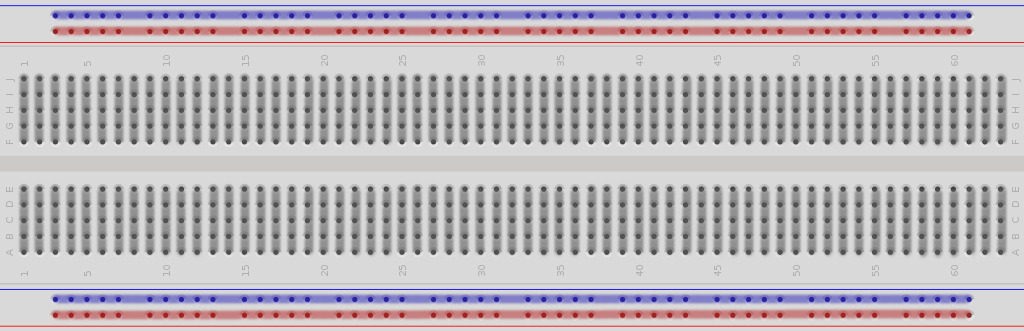
\includegraphics[width=0.8\textwidth]{protoboard_connections}
\caption[Typical connections on a prototyping board]{Typical connections on a
prototyping board. The holes adjacent to each of the red and blue lines are
connected to each other, as indicated by the red and blue highlights on
the figure. The remaining holes are connected in groups of five, as indicated
by the grey highlights.}
\label{fig:protoboard_connections}
\end{figure}

As an example, let's consider how we might wire together a simple circuit 
involving a 9 volt battery and an LED using a protyping board. Note that 
nine volts is usually a little high for powering a single LED, so we are also
going to put a resistor in our circuit to keep the current down.

First, let's connect our battery to the red an blue rows of the 
prototyping board. You don't necessarily have to connect the power this way 
(in fact, once you know how the connections in the prototyping board work, you
can connect things in any fashion consistent with the circuit you are trying 
to build), but doing so is generally considered good practice. We can also
connect each set of row together, so that we are providing a power 
source and ground at both the top and bottom of the board. As you know, the
color of the wires I use doesn't make any difference in how the circuit 
operates, but the colors \textit{can} help me keep track of how I've built my
circuit. Red is typically used for power sources, and dark blue or black is
typically used for ground (or the negative terminal for DC sources). Once I've
made these connections, my prototyping board looks like Figure
\ref{fig:protoboard_example_a}.
\begin{figure}[hbp!]
\centering
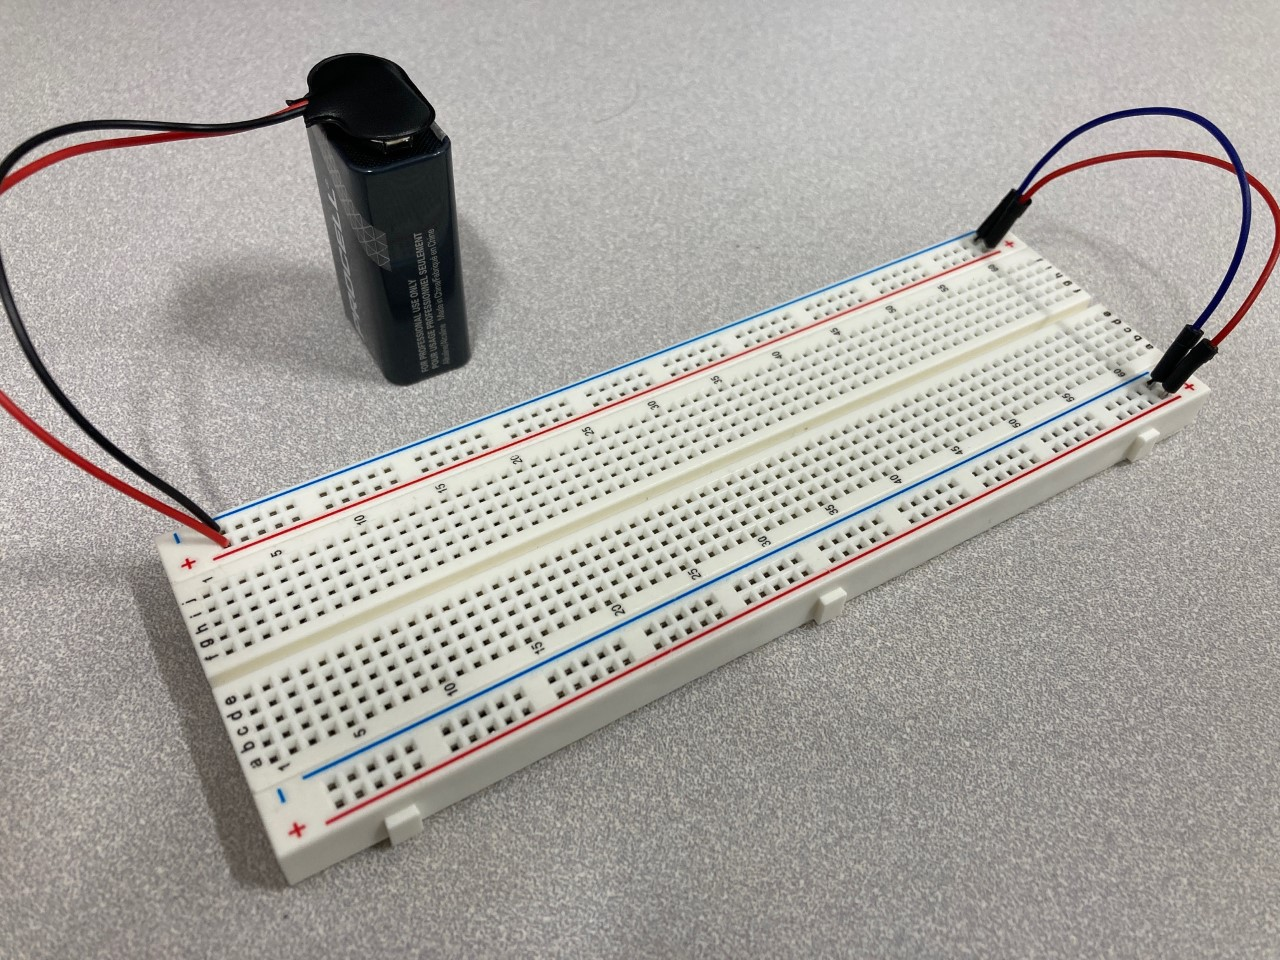
\includegraphics[width=0.8\textwidth]{protoboard_example_a}
\caption[Connecting power to a prototyping board]{Connecting power to a 
prototyping board. Note that the positive lead from the battery holder
connects to the ``red'' horizontal line on the prototyping board, and the
negative lead (the black wire) connects to the ``blue'' line. The red and
blue wires on the right side connect the two red and blue lines together,
respectively.}
\label{fig:protoboard_example_a}
\end{figure}

Our next step is to connect the LED to the red power row. LEDs are picky 
about which lead is connected to power. One of the leads will be longer than the
other. This is the lead that should connect to the power. For our circuit, I 
will plug this long lead directly into one of the holes I've provided power to,
and the other lead into one of the center strips, as seen in Figure
\ref{fig:protoboard_example_b}.
\begin{figure}[hbp!]
\centering
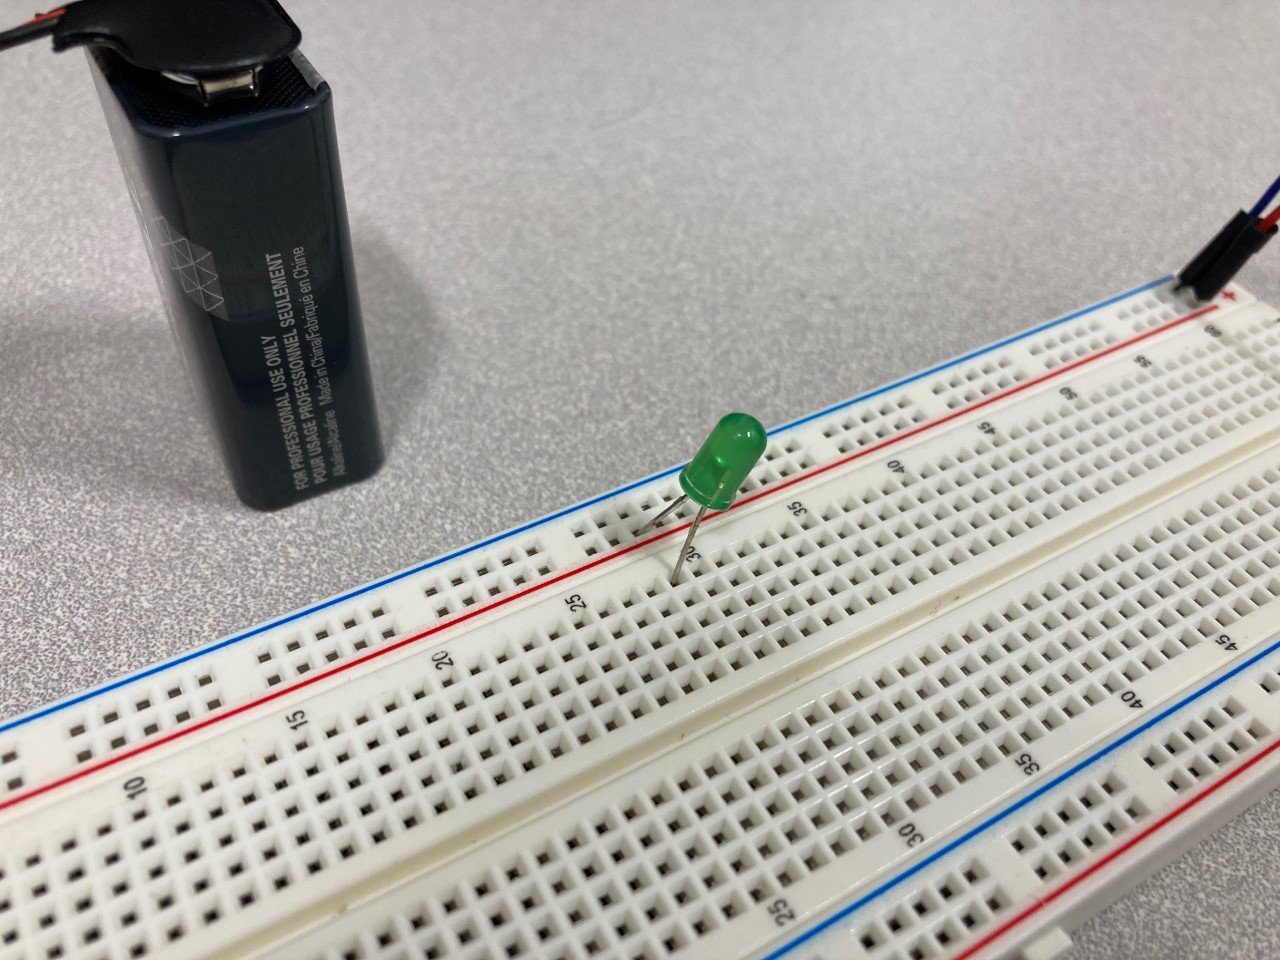
\includegraphics[width=0.8\textwidth]{protoboard_example_b}
\caption[Adding an LED to the prototyping board]{Adding an LED to the 
prototyping board. The long lead is placed in one of the holes connected
to power, and the other lead is connected to a center strip.}
\label{fig:protoboard_example_b}
\end{figure}

At this point, our LED has not lit, because it needs to form a complete circuit,
which we could do by connecting a wire from the unconnected lead to ground
(one of the blue rows). We don't want to do this, though, as the full nine
volts from the battery is probably too much for our LED. So we're going to put
a resistor in first. I'll use a 330 Ohm resistor for this exercise. I connect
one of the resistor leads into the same five hole group that the LED is 
connected to, and the other lead into a hole from a different group (putting
both leads into holes from the same group would be like connecting the two
ends of the resistor together, effectively removing it from the circuit). These
connections can be seen in Figure \ref{fig:protoboard_example_c}.
\begin{figure}[hbp!]
\centering
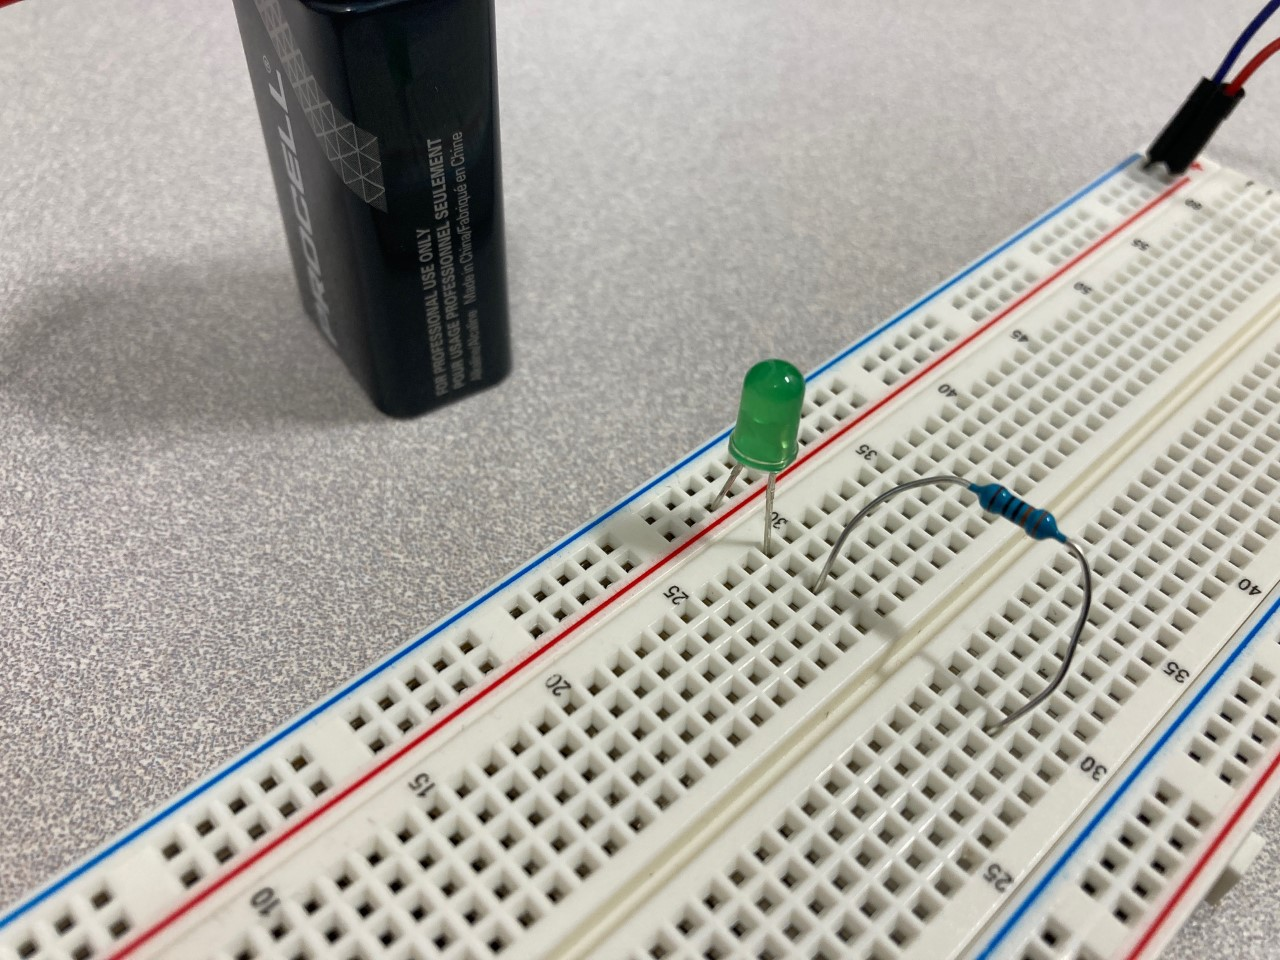
\includegraphics[width=0.8\textwidth]{protoboard_example_c}
\caption[Adding a resistor to the prototyping board]{Adding a resistor to the
prototyping board. One lead is placed in one of the holes in the same group
as the LED lead, and the other lead is connected to a different group.}
\label{fig:protoboard_example_c}
\end{figure}

Our LED is still not lit. We will now complete the circuit by adding a ground
connection. I could have done this by putting the second lead of the resistor
into one of the ground holes, but I'll instead use a wire to finish the
connection. The LED is now lit (Figure \ref{fig:protoboard_example_d})!
\begin{figure}[hbp!]
\centering
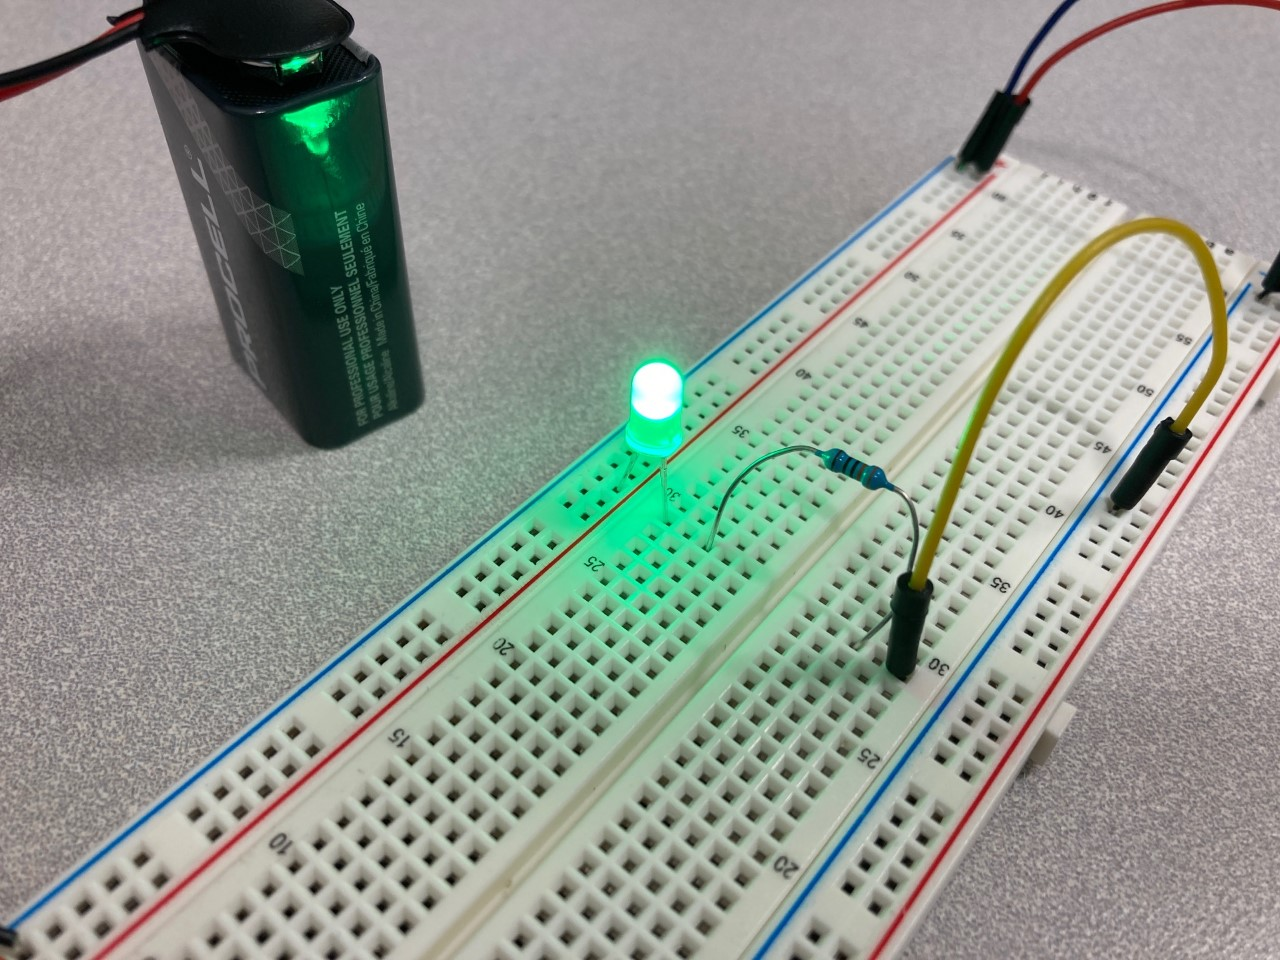
\includegraphics[width=0.8\textwidth]{protoboard_example_d}
\caption[Completing the simple LED circuit]{Completing the simple LED circuit.
One end of the yellow wire is connected to the same group as the end of the
resistor, and the other end of the wire is connected to the ground (blue)
row. Having completed the circuit, the LED is lit.}
\label{fig:protoboard_example_d}
\end{figure}

\activity{
With the exception of the 9 V battery, build the circuit from this example
on a prototyping board.
}

This concludes our example for using a prototyping board to construct a circuit.
Before this lab concludes, we are going to use our Arduino as the power source
for this circuit, and also have a little fun using the Arduino to control the
behavior of the LED. Before we do that, though, we need to talk about soldering.

\subsection{Durable circuits: soldering}

If you followed the last example carefully, you may have 
noted a few things:
\begin{itemize}
\item Using the prototyping board makes this circuit a lot larger than it 
needs to be.
\item We made electrical connections by easily sliding a lead or wire into a
hole. The wire or lead can just as easily be removed from the hole.
\item The entire thing looks like it will fall apart if I try to pick it up
and move it.
\end{itemize}
It is fairly apparent that prototyping boards are good for designing circuits
and building a prototype for testing (hence the name ``prototyping board'').
But if I am going to put this circuit to any sort of practical use, I need to
build it in a more permanent fashion. The way we do this is by electrically
``gluing'' the connections together with solder.

Solder consists of a ductile metal alloy (usually tin, silver, and/or lead) 
mixed with a small amount of material called flux. Solder has a relatively low
melting point, and is also electrically conductive. By melting a little bit of
solder between the wires or leads we want to connect, and then letting the 
solder reset, we can make a mechanically strong connection.

In order to make a mechanically strong and electrically sound connection, 
soldering must be done correctly. The process begins by making sure you have
the right equipment and that it has been properly prepared. Figure
\ref{fig:soldering_equipment} shows the elements of a good soldering station, 
including (from left to right)
\begin{itemize}
\item A soldering iron. This provides the heat to melt the solder.
\item Solder. In this case, it is provided on a spool.
\item Flux paste. Flux is what helps solder flow. Sometimes solder doesn't
have enough flux, and having a little extra paste handy can make a huge 
difference.
\item Tip cleaner. The tip of a soldering iron, after a little use, will start
get gummed up with oxides. When this happens, it doesn't conduct heat very well.
Frequent tip cleaning makes your life a lot easier!
\item Helping hands. This device includes a few clamps that can hold your work
in place, and usually also includes a magnifying glass to help you see what
you are doing. This piece of equipment is critical! Normally, when soldering a
circuit, you need to hold the circuit, the element you are soldering to it, 
the soldering iron, and the solder all at the same time. Unless you have four
hands, you'll need one of these devices!
\item Wire wick. Sometimes you make mistakes while soldering. Wire wick, when 
heated, will sop up solder so you can remove it from your work.
\end{itemize}
\begin{figure}[hbp!]
\centering
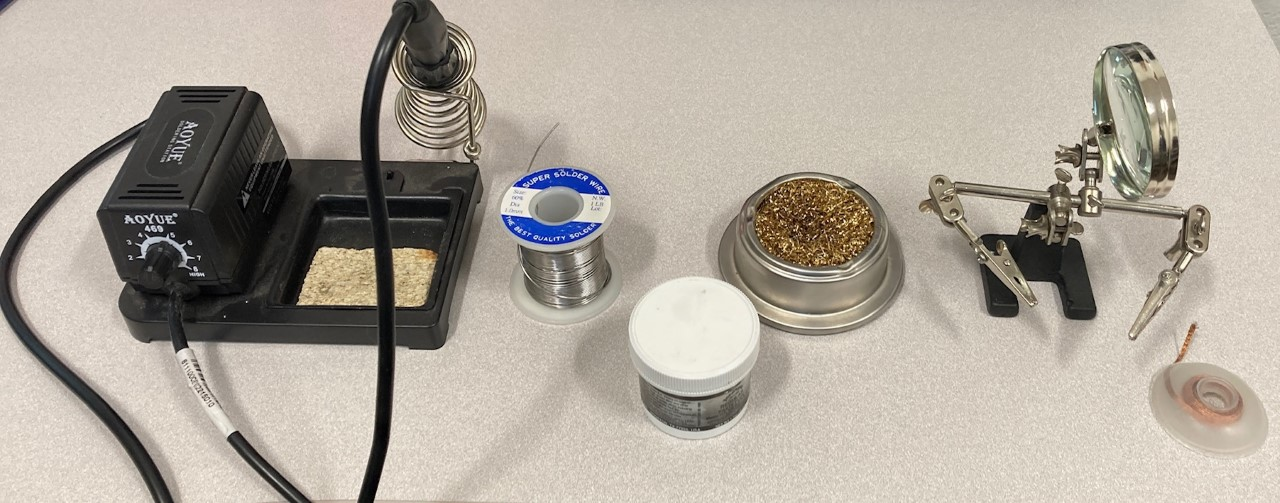
\includegraphics[width=0.8\textwidth]{soldering_equipment}
\caption[Soldering equipment]{Soldering equipment. Included here are
a soldering iron, solder, flux paste, a tip cleaner, a set of ``helping
hands'', and wire wick. See the text for a more full description of these
items.}
\label{fig:soldering_equipment}
\end{figure}

In addition to this equipment, it's also convenient to have a surface to 
solder our components on, rather than trying to solder them together directly.
A common surface is pictured in Figure \ref{fig:perfboard}, and is called a
perfboard. It's basically just a fiberglass board with a bunch of holes
(perforations) drilled in it, and the holes are lined with some sort of 
conductive material.
\begin{figure}[hbp!]
\centering
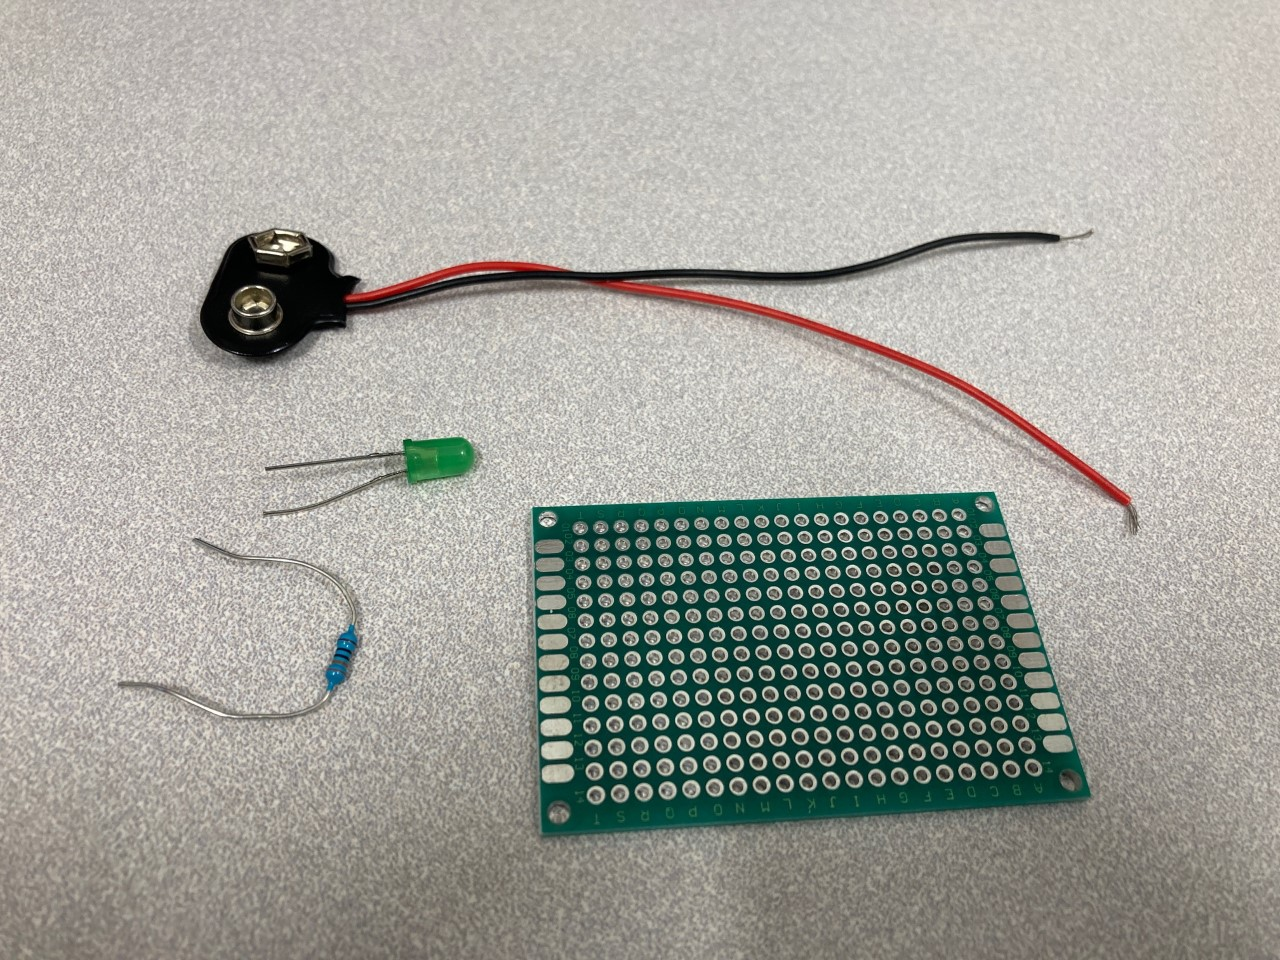
\includegraphics[width=0.8\textwidth]{perfboard}
\caption[A perfboard]{A perfboard, along with some items we will solder
together on it.}
\label{fig:perfboard}
\end{figure}

Now, let's get started. First we'll plug the soldering iron in and give it a 
few minutes to heat up. Once heated, we then want to clean and prepare the tip.
This is done by plunging the tip of the soldering iron in and out of the tip 
cleaner several times. At this point, we'll also dip the tip very briefly 
into the flux paste, and then clean the tip again. Finally, we'll melt a small 
amount of solder onto the tip, and then clean it a third time. At this point,
the tip should be clean and shining with solder, similar to Figure
\ref{fig:solder_ready}.
\begin{figure}[hbp!]
\centering
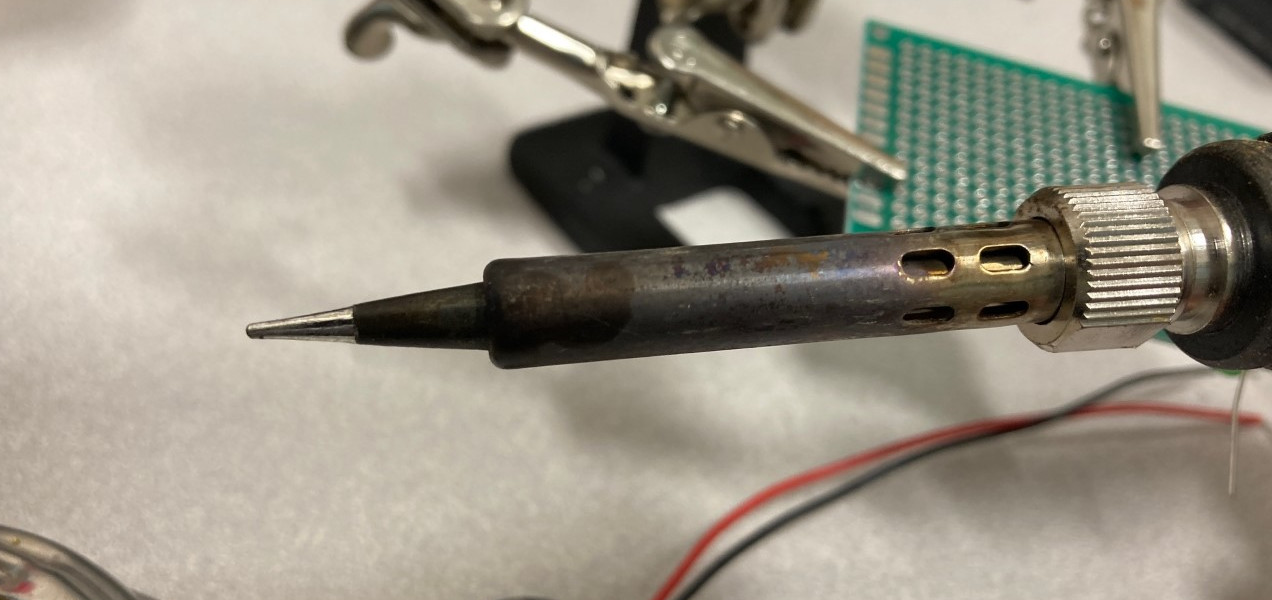
\includegraphics[width=0.8\textwidth]{solder_ready}
\caption[A clean soldering iron tip]{A clean soldering iron tip, ready for
use.}
\label{fig:solder_ready}
\end{figure}

The next step is to start putting elements on the perfboard. Components with
leads can usually be held in place prior to soldering by bending the leads on
the backside of the board. These bent leads can also conveniently be used as
wires between components as well. In Figure \ref{fig:component_preparation},
all of the components for the circuit have been placed on the boards, and 
the leads bent to make electrical connections. Normally you would only add a 
few components at a time, solder those into place, then add more.
\begin{figure}[hbp!]
\centering
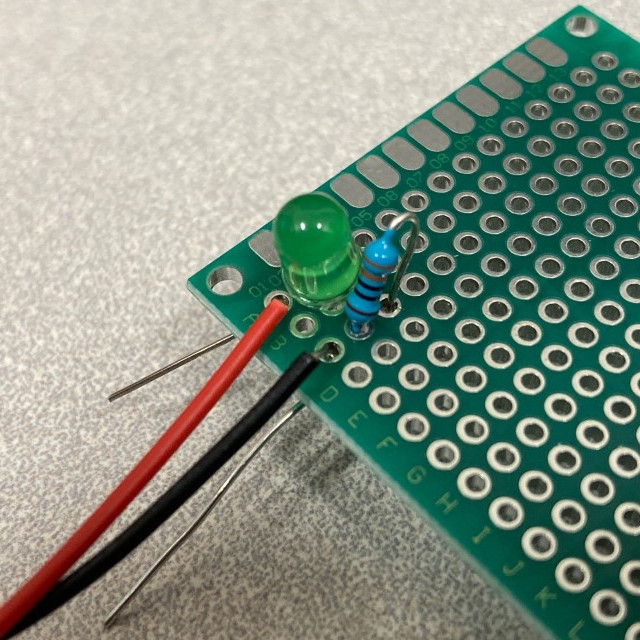
\includegraphics[width=0.4\textwidth]{component_preparation_a}
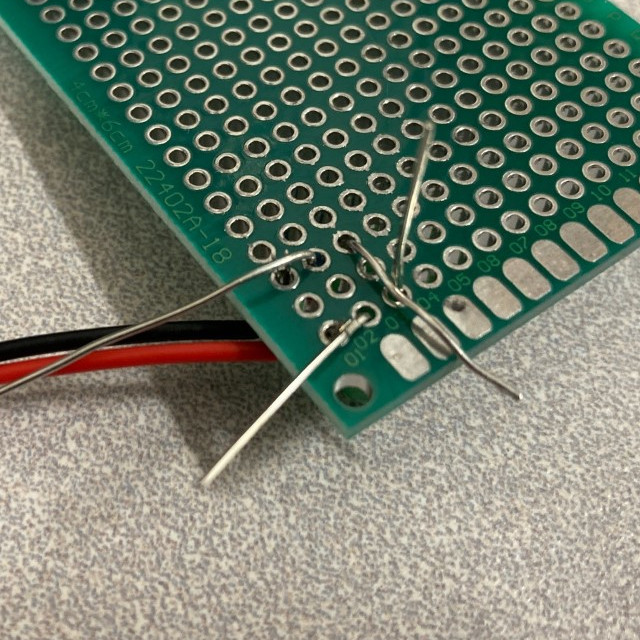
\includegraphics[width=0.4\textwidth]{component_preparation_b}
\caption[Components added to a perfboard, ready for soldering]{Components added
to a perfboard, ready for soldering. Note how, on the back side of the 
perfboard, the leads have been bent to hold the components in place as well as
act as wires.}
\label{fig:component_preparation}
\end{figure}

Now to apply the solder. Rather than trying to hold the entire spool of 
solder, it's easiest to use the soldering iron to burn off a three or so inch
segment instead. A key thing to remember is that you should
\textit{\textbf{heat the work, not the solder}}. If you just touch the solder
with the soldering iron, it will melt, and it might even transfer onto the
parts you are trying to solder. However, the flux tends to move to the 
surface of hot metal, and you'll basically end up with a ball of solder that
is insulated from the work by a thin layer of flux. This is referred to as a
\textit{cold solder} joint, and will likely not provide a lasting electrical
connection. By heating the work and then melting the solder onto the work,
you'll end up with good connections. 
\begin{figure}[hbp!]
\centering
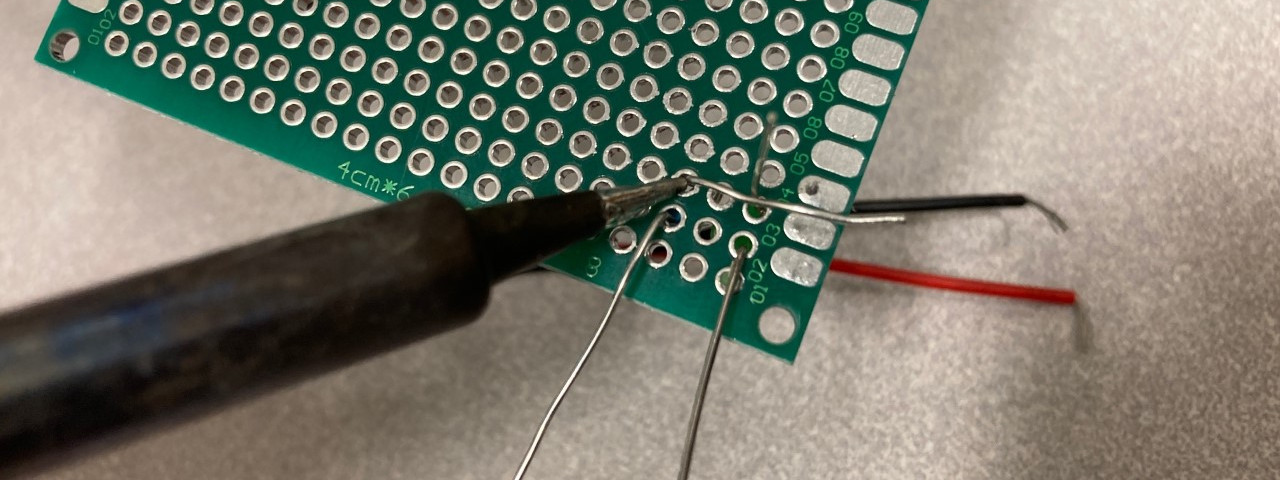
\includegraphics[width=0.8\textwidth]{heat_the_work}
\caption[Heat the work, not the solder!]{Heat the work, not the solder!}
\label{fig:heat_the_work}
\end{figure}

Once the iron is removed from the working area, the solder will cool and set
very quickly.
This process is repeated for each of the
connections. Figure \ref{fig:soldering_almost_done} shows the results with just
a few connections left to solder. In this figure, you'll note that one of the
clamps on the helping hands is holding the wire in place.
\begin{figure}[hbp!]
\centering
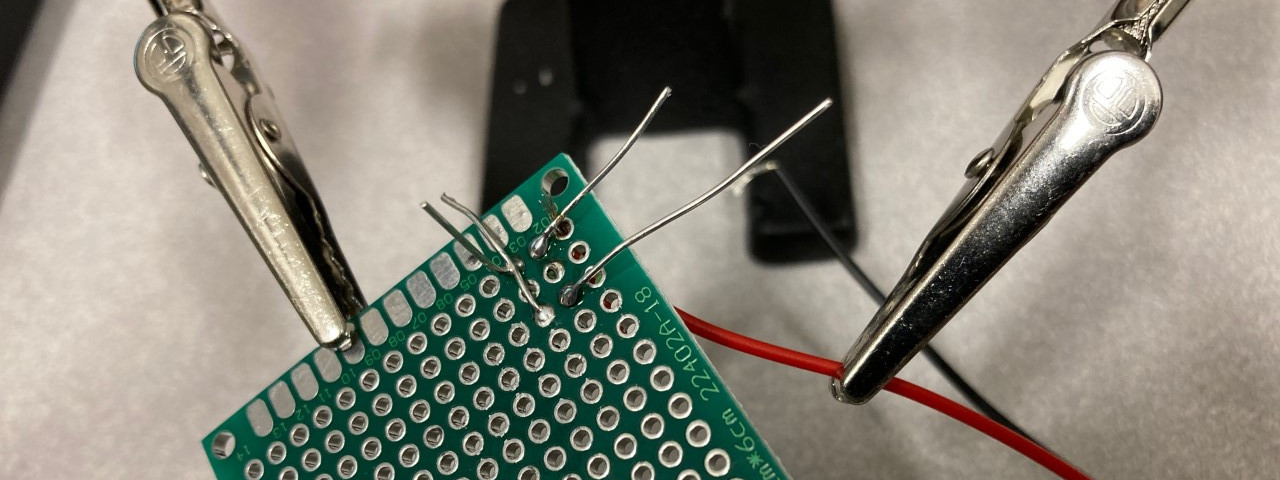
\includegraphics[width=0.8\textwidth]{soldering_almost_done}
\caption[Soldering project near completion]{The soldering project near 
completion. The connections to the 9 V battery connector still need to be
soldered. Note that one of the clamps of the helping hands is holding the red
wire in place.}
\label{fig:soldering_almost_done}
\end{figure}

Once all of the soldering is complete, you'll have some tails of wire and
component lead sticking out. Use a set of close clipping wire cutters to remove
these extra and unnecessary pieces of metal. Now our project is complete
(see Figure \ref{fig:soldering_complete}. Note that the finished product is
significantly more durable than what we had on the prototyping board, and also
significantly smaller. (The perfboard used here is 4 cm by 6 cm, and clearly a much smaller board could have been used.
\begin{figure}[hbp!]
\centering
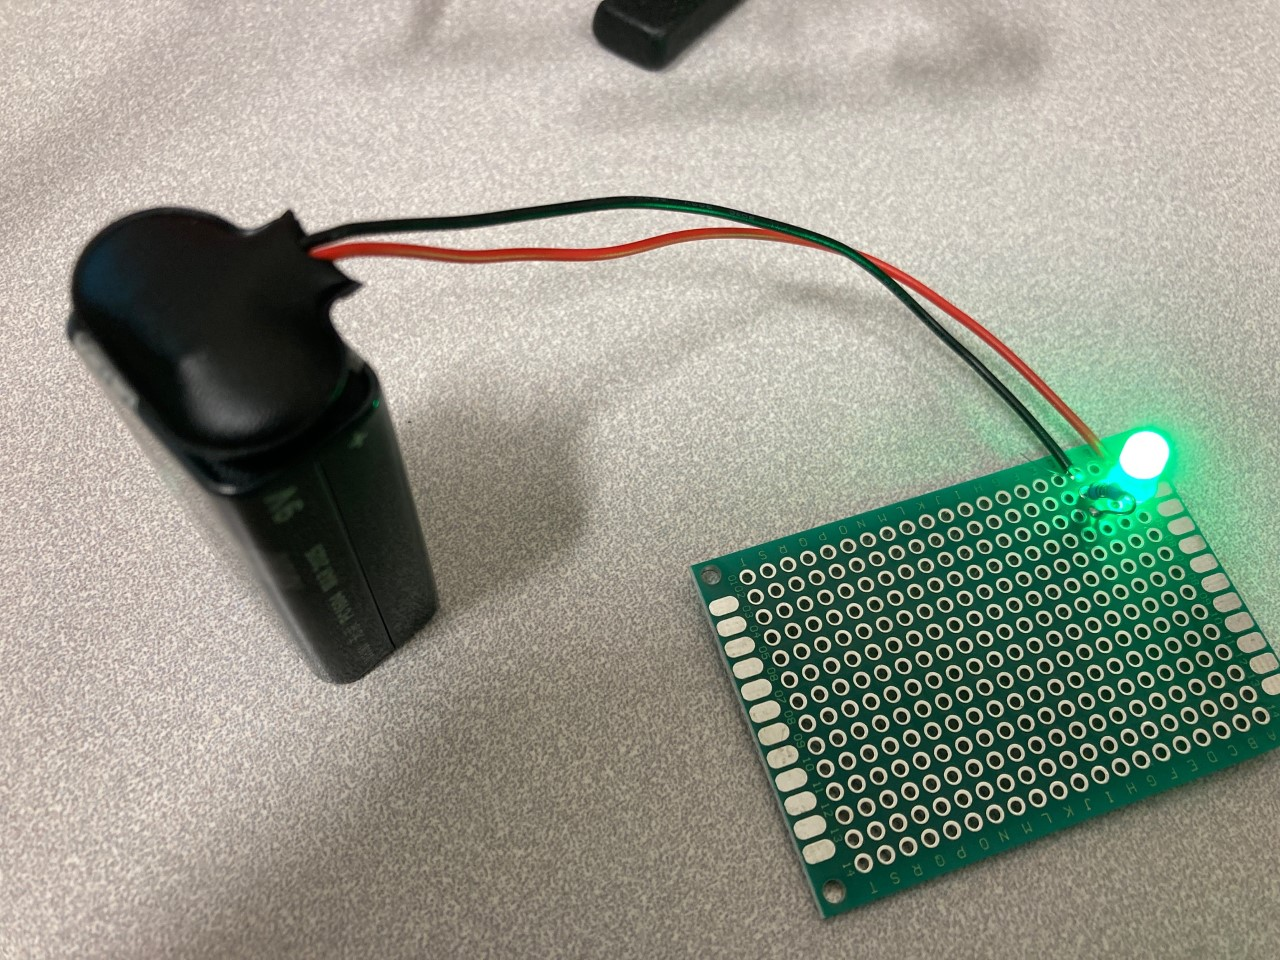
\includegraphics[width=0.8\textwidth]{soldering_complete}
\caption[The completed soldering project]{The completed soldering project.}
\label{fig:soldering_complete}
\end{figure}

When a particular circuit needs to be produced in large amounts, someone will
usually design and produce a printed circuit board, or PCB. A PCB consists of 
several layers of conductors, insulating substrates, and inks. The conducting
layers make the connections between circuit elements, so one only needs to
solder the circuit elements in place, and not worry about wiring the 
connections between them. An example of a PCB can be seen in Figure
\ref{fig:pcb}. The conducting layers are most obviously visible in the
lower left portion of the PCB.
\begin{figure}[hbp!]
\centering
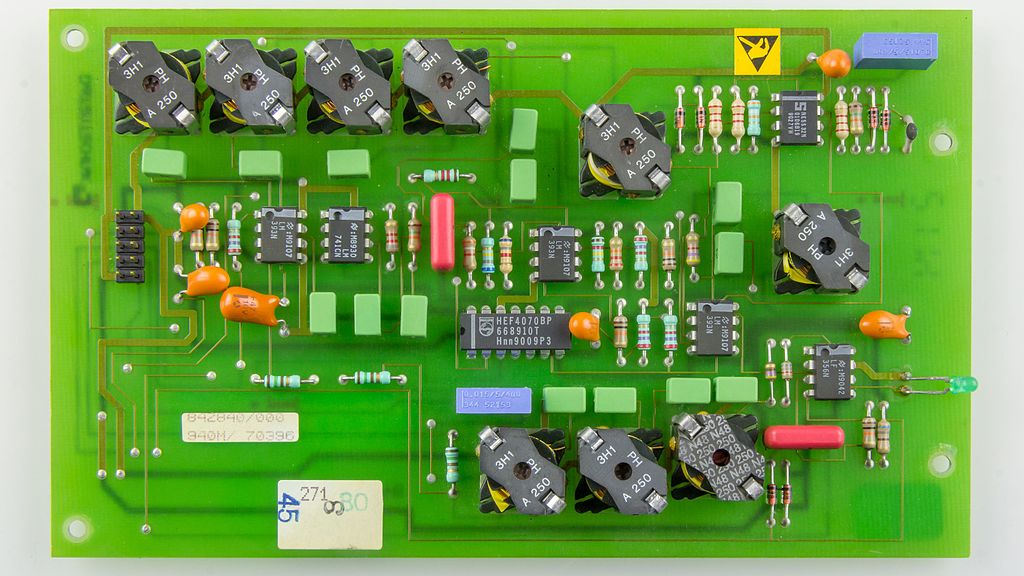
\includegraphics[width=0.8\textwidth]{pcb}
\caption[A printed circuit board]{An example of a printed circuit board,
populated with components. The conducting layers are highly visible in the 
lower left portion of the board.}
\label{fig:pcb}
\end{figure}

The type of soldering presented here is called ``through hole'' soldering, so 
named because leads from the components are placed through holes and then
soldered into place. Smaller circuit elements are often soldered directly to
pads on the surface of a PCB. This type of soldering is called ``surface
mount'', and is somewhat more difficult to perform. We will not be doing any
surface mount soldering in this lab. Both through hole and surface mount
connections can be seen in Figure \ref{fig:pcb}. The diodes, resistors, and
inductors (all cylindrically shaped components with one or more bands around 
their circumferences) have been connected with through hole soldering. The
ICs (the black boxes) are connected via surface mount.

\activity{
Successfully complete three or more soldering connections.
}

Now that we've seen how to design, build, and solder circuits, let's look at
controlling our circuit using an Arduino.

%%%%%%%%%%%%%%%%%%%%%%%%%%%%%%%%%%%%%%%%%%%%%%%%%%%%%%%%%%%%%%%%%%%%%%%%%%%%%%%%

\section{Arduino Circuit Control}

Let's start our study of computer control by controlling something simple
with an Arduino DAQ: the LED circuit that we constructed earlier on the
prototyping board. Our objective is to use the Arduino to turn the LED on and 
off. 

\subsection{Attaching the Arduino to the circuit}

Connecting the Arduino to our LED circuit built earlier is quite simple. We 
will be using the digital I/O ports found on one side of the Arduino, as 
seen in Figure \ref{fig:arduino_left}. In this figure, you will see that 
these ports are numbered, starting from the left, 1-13, GND, AREF, SDA, and
SCL. Of those ports, the ones of greatest interest to us today are the numbered
ports and the GND port (GND stands for ``ground''). The numbered ports will be
our voltage source, and the GND port will be our ground connection (akin to the
negative terminal of a battery).
\footnote{You will note that the
Arduino is assembled on a printed circuit board. Can you identify which 
components were attached by through hole v. surface mount soldering?}
\begin{figure}[hbp!]
\centering
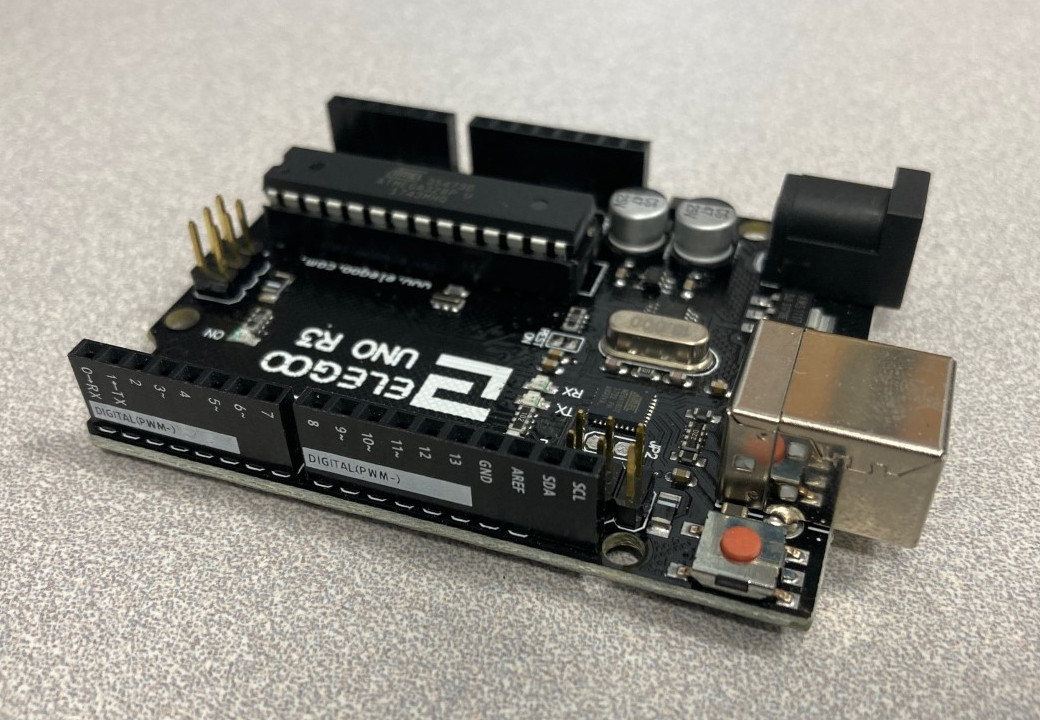
\includegraphics[width=0.8\textwidth]{arduino_left}
\caption[The digital ports on an Arduino]{The digital ports on an Arduino.}
\label{fig:arduino_left}
\end{figure}

To connect the Arduino to our circuit, we place a wire into port 13 (or any
of the other numbered ports, but for the example here we're going to use port
13), and the other end of the wire into the red row of our prototyping board.
This is the same way we connected the positive terminal of the battery earlier.
A second wire connects the GND port of the Arduino to the blue row, where we
had previously connected the negative terminal of the battery. These 
connections can be seen in Figure \ref{fig:arduino_connected}.
\begin{figure}[hbp!]
\centering
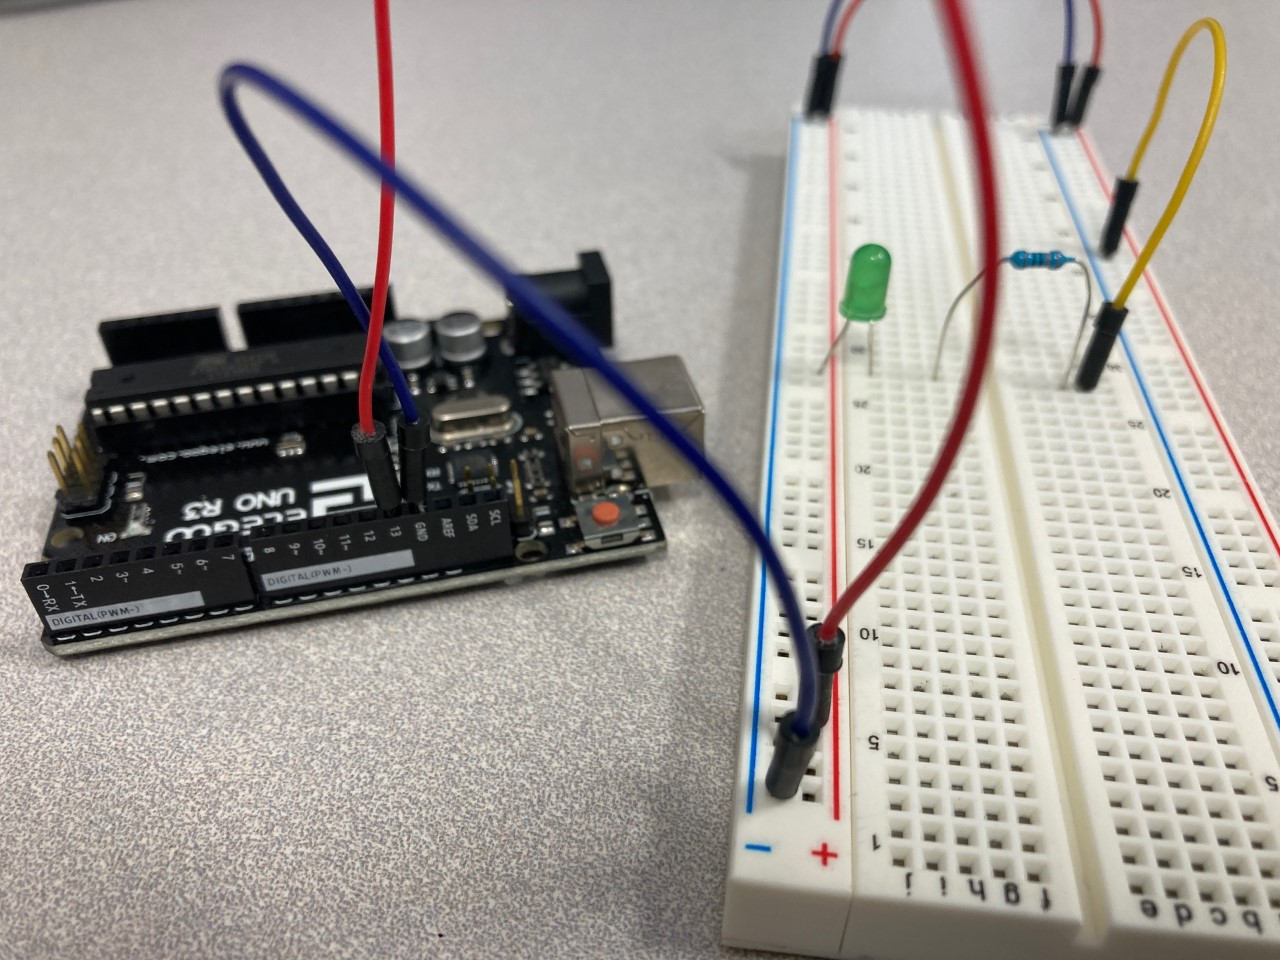
\includegraphics[width=0.8\textwidth]{arduino_connected}
\caption[The Arduino connected to the LED circuit]{The Arduino connected to
the LED circuit. The connections are described in the text.}
\label{fig:arduino_connected}
\end{figure}

A discussion about ``ground'' is warranted here. The name ``ground'' is quite
literal, in a way. The Earth is big, and can act as a giant sink for electric
potential. More importantly for us, the ground provides a reference that we
can measure electric potentials with respect to. The numbered ports on the
Arduino are going to provide five Volts of potential relative to ground. How 
does the Arduino know what the ``ground'' is? Because it will also be connected
to our computer. The plug on our computer has a ``ground'' prong (the round
prong), which (if the building you are in is wired to applicable codes) is 
electrically connected to a copper rod that has been pounded down into the
ground.

From this point on, we will no longer provide pictures of the circuits that
we build (usually). Circuits are typically represented using schematic diagrams
instead of pictures. A schematic diagram is a simplified representation of
a circuit. Each type of component has a symbol associated with it. Connections
between components are represented with lines. Connections to things outside
of the circuit are represented by pins. As an example, the circuit we have
just built is represented in Figure \ref{fig:blink_circuit}. The rectangle 
labeled with ``R1'' is our resistor, and you can see the resistance value
next to the label. The arrowhead terminating on a line, labeled ``D1'', 
represents a diode. The smaller arrows leaving the diode indicate that this 
is a light emitting diode, or LED (also indicated by the label). The pinouts to 
the Arduino are labeled ``J1'' and ``J2'', and their intended connections are
also included on their labels. Part of the fun of building electric circuits is 
constructing a physical circuit 
from the information given in the schematic!
\begin{figure}[hbp!]
\centering
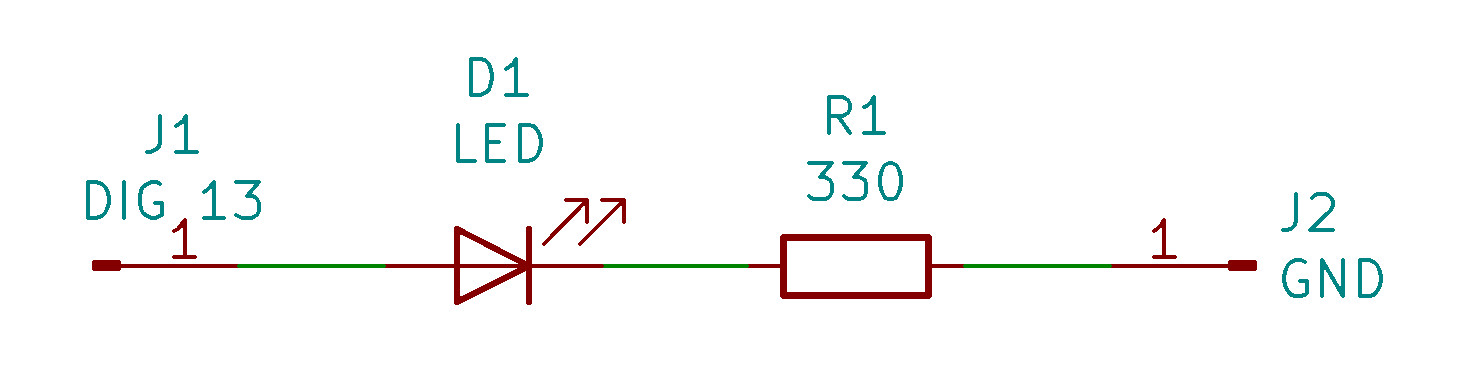
\includegraphics[width=0.8\textwidth]{blink_circuit}
\caption[Schematic diagram for the blink circuit]{Schematic diagram for the
blink circuit. The rectangle symbol represents the resistor, and the other
symbol represents the LED. The pinouts to the Arduino are labeled at the ends.
See the text for a more full description.}
\label{fig:blink_circuit}
\end{figure}

At this point, the LED is still out. There are two reasons for this. First, we
have not yet provided power to the Arduino. Second, we have not yet told the 
Arduino to turn on the LED. Providing power to the Arduino can be done in
several ways. For today, we will simply connect the Arduino to our computer
using a USB cable. (We need this USB connection in order to program the
Arduino, also.)

\subsection{The Arduino sketch: an introduction}

We now have our ``hardware'' built for a blinked LED. We still need to 
give instructions to our Arduino so it knows how to use pin 13 and GND to
make the LED blink. The Arduino has a small computer on board, and we need
to upload a computer program to the Arduino in order to tell it what to do.

You have likely already written programs at some point in your education. 
Common programming languages include Python, Java, and C++. Arduino programs
are similar to other programming languages\footnote{The Arduino programming
language is essentially C++ with some modification. If you are already familiar
with C or C++, Arduino programming will feel quite comfortable.}. 
They have loops and conditional statements, but additionally have special code
for controlling the Arduino.

Most Arduino codes are very short. For today's code, we just need to tell the
Arduino what to turn on and when, and when to turn it back off again.

Every Arduino program has two required parts: the \code{setup()} function and
the \code{loop()} function. When the Arduino is powered on, the \code{setup()}
function is executed once. As the name of the function implies, it is typically
used to set up variables or environments that the rest of the program will use.
Once the \code{setup()} function has been executed, the \code{loop()} function
is executed. This is where most of the action happens in the program. This 
function is repeated over and over again until the Arduino is powered down.

Let's introduce the commands we will use for this lab. Each digital output on
the Arduino has a number. The code will need to know which pin number we are
working with. There are two ways we can do this. The first is to define a 
variable of type integer (int) and set it equal to the pin number. The code to
do this would typically be written before the \code{setup()} function, and 
would look something like this:
\begin{lstlisting}[language=Arduino] 
int ledPin=13;
\end{lstlisting}
The other way we can do this is with a \code{\#define} 
statement at the beginning of the code,
before the \code{setup()} function.
A \code{\#define} statement 
simply tells the compiler (the thing that turns our human
readable code into binary code that the processor understands) to replace the
defined name with whatever follows in the definition. Such a definition would
look something like this:
\begin{lstlisting}[language=Arduino] 
#define ledPin 13
\end{lstlisting}

As stated before, most of the action of the program happens in the
\code{loop()} function. In our case, our loop function needs to turn on
the digital pin our LED is connected to, wait for a short while, turn it off
again, and then wait some more.
A digital pin on the Arduino can be set to a LOW voltage (zero Volts relative
to ground) or a HIGH voltage (+5 V relative to ground). Each digital pin that
we use also needs to be set up for output or input. This is done with a 
``pinMode'' statement. For example, to set pin 13 to output, I would use the 
following in my \code{setup()} function, recalling that we had previously
set \code{ledPin} to a value of 13:
\begin{lstlisting}[language=Arduino] 
    pinMode(ledPin,OUTPUT);
\end{lstlisting}
If I had wanted to set up the pin for input, I would simply replace the
\code{OUTPUT} with \code{INPUT}.

To set the pin to LOW or HIGH voltage, use a digitalWrite command:
\begin{lstlisting}[language=Arduino] 
    digitalWrite(ledPin,LOW);
    digitalWrite(ledPin,HIGH);
\end{lstlisting}
And, finally, to leave the light on (or off) for a while, we can use
a delay command, where the argument to the command gives the delay time in
milliseconds:
\begin{lstlisting}[language=Arduino] 
    delay(100);
\end{lstlisting}

Altogether, our Arduino code for blinking lights would read as follows:
\begin{lstlisting}[language=Arduino] 
#define ledPin 13

void setup() 
{
    pinMode(ledPin, OUTPUT);
}

void loop() 
{
    digitalWrite(ledPin,HIGH);
    delay(100);
    digitalWrite(ledPin,LOW);
    delay(100);
}
\end{lstlisting}
There are a few things to note about the syntax. First, every line of command
within the code is terminated with a semicolon. This tells the compiler that the
command is complete, and also allows us to continue a command onto a second
or third line when needed. The only exception is the \code{\#define} statement.
Second, any grouped set of command, be that in a function, a loop, or a 
conditional statement (the latter two do not appear in this code) are 
encapsulated in a set of curly braces. Once again, this tells the compiler 
where the set of commands begins and ends.

The code above, while it will make the Arduino behave the way we want, is not
ideal. It is missing a \textit{\textbf{very critical}} part: comments. You 
should always include abundant comments in your code, including a comment 
block at the top describing what the code does overall, comments describing
each variable you declare or define, and comments that describe each part of
the algorithm in the code. Why do you want so many comments? Some people would
say that you include comments to help other people understand what your code
is doing. The reality is, though, that you put the comments in your code so 
that \textit{\textbf{you}} can remember what your code is doing when you 
come back to it weeks or months later. For this lab course, comments are 
required in all of your code.

In the Arduino language, single line comments can be started with a double
forward slash ``//''. Block comments can also be started with a ``/*'' and 
ended with a ``*/''.
Once I've included adequate comments, my code will look something like this
\begin{lstlisting}[language=Arduino] 
/////////////////////////////////////////////////////////
// Arduino sketch to blink one LED
//   Written by (your name would go here)
//   Feb. 6, 2017 
/////////////////////////////////////////////////////////

// Define the pin we are using for output

#define ledPin 13

/////////////////////////////////////////////////////////
// The arduino setup function comes next. We need to set
// up pin 13 for output. 
/////////////////////////////////////////////////////////

void setup() 
{
    pinMode(ledPin, OUTPUT);
}

/////////////////////////////////////////////////////////
// Now comes the loop function. We simply turn on the 
// LED, wait for a while, turn off the LED, and wait 
// some more.
/////////////////////////////////////////////////////////

void loop() 
{
    digitalWrite(ledPin,HIGH);  // Turn on the LED
    delay(100);                 // Wait 100 ms
    digitalWrite(ledPin,LOW);   // Turn off the LED
    delay(100);                 // Wait 100 ms
}
\end{lstlisting}

\subsection{Compiling and uploading the sketch}

So that's how you write Arduino code. How do you get it to your Arduino? 
There is a special integrated development environment (IDE) for 
programming our Arduino. The IDE can be seen in Figure \ref{fig:ide}.

We will need to install this IDE before we can communicate with our 
Arduino. To do so we use a web browser to go to\\

\href{https://www.arduino.cc/en/Guide/HomePage}{https://www.arduino.cc/en/Guide/HomePage}\\

\noindent and choose to install the Arduino IDE for your computer. 
In the figure, you will see two important buttons on the left side of the 
toolbar. One is the ``compile'' button. The Arduino cannot interpret the 
human readable code that we write in the IDE. It needs to have the code 
translated into binary (ones and zeroes) that digital logic circuits understand.
This translation process is called ``comiling''. As the code is compiled, the
Arduino software looks for errors in the code. If there are errors, it will
tell you at this point. This way we can correct the errors before we send 
the compiled instructions to the Arduino.
\begin{figure}[hbp!]
\centering
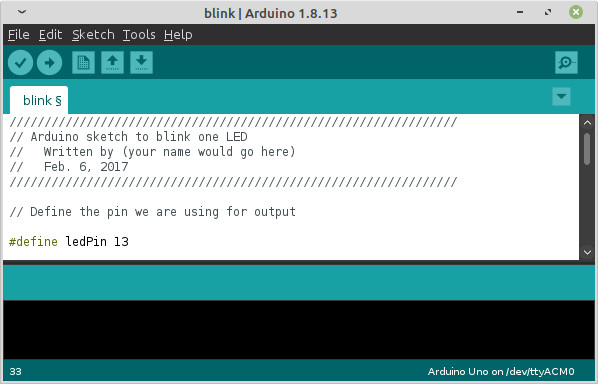
\includegraphics[width=0.8\textwidth]{ide}
\caption[The Arduino IDE]{The Arduino IDE. The compile and upload buttons are
found at the left side of the tool bar.}
\label{fig:ide}
\end{figure}

We also need a way to send our code to our Arduino and that is what the
upload to Arduino button does. Once the code is compiled without errors,
connect the USB\ cable to the Arduino and push the upload button. Once the 
code is uploaded to the Arduino, we should see some blinking lights!

One last thing to note: Arduino programs are called ``sketches''. As you 
keep your lab notebook, you should always include a copy of your sketch, along
with notes on how you got it to work. It's also a good idea to include 
pictures and schematics of any circuits you have constructed.

\activity{
Build your own clone of the blinking light circuit described in this section
by doing each of the following:
\begin{itemize}
\item Construct the LED circuit on a prototyping board.
\item Connect the Arduino to the LED circuit and to your computer.
\item Write, compile, and upload the ``blink'' sketch to the Arduino.
\item Verify that the circuit is working correctly.
\end{itemize}
}

%%%%%%%%%%%%%%%%%%%%%%%%%%%%%%%%%%%%%%%%%%%%%%%%%%%%%%%%%%%%%%%%%%%%%%%%%%%%%%%%

\section{Adding More Complexity}

Now it's your turn to practice these skills by designing a building a new
circuit. Our objective is to build an Arduino
controlled circuit that does the following:
\begin{itemize}
\item Increments a counter every half second.
\item Turns on a red LED only when the counter is an even number.
\item Turns on a yellow LED only when the counter is a multiple of three.
\item Turns on a green LED only when the counter is a multiple of five.
\item Turns on a blue LED only when the counter is a multiple of seven.
\end{itemize}
Most of hardware setup will be the same, but we will be using multiple
digital pins on the Arduino (one for each LED). We will have to abandon our 
nice $+5\unit{V}$ top row on our prototyping board as our connection to
pin 13, because we need multiple pins and we need them to operate independently.
Instead, we can wire pin 13 of our Arduino directly to the top lead of one LED, 
wire pin 12 to the top lead of another LED, and so on. It's OK for each branch
of this circuit to share the same ground connection.

To do this, we will need a counter variable. The variable \code{i} is a common
choice. You'll want to declare this variable as an integer at the beginning of
your sketch, and set its value equal to zero. At the end of the loop statement,
you can increment the counter using 
\begin{lstlisting}[language=Arduino]
    i=i+1;
\end{lstlisting}
or
\begin{lstlisting}[language=Arduino]
    i++;
\end{lstlisting}

You will also need to make the Arduino to some math. Specifically, you'll need
to test whether the counter is currently a multiple of the desired number.
This can be done using a conditional statement. In the Arduino language, 
conditional statements will take on the following form:
\begin{lstlisting}[language=Arduino] 
    if(a<b)
    {
        firstFunction();
	delay(100);
	secondFunction();
    }
    else if(a<c)
    {
        anotherFirstFunction();
	delay(200);
    }
    else
    {
        finalFunction();
    }
\end{lstlisting}
Each part of the condition includes a test statement found in the parentheses.
If the statement is true, the code included in the curly braces that follow
will be executed. In this example, if \code{a>b} evaluates true, then the
\code{firstFunction}, \code{delay}, and \code{secondFunction} will be 
executed in order. It will then skip over the rest of the code in the example.
If \code{a>b} evaluates false, the code will procede to the \code{else if}
portion of the conditional, executing the \code{anotherFirstFunction} and 
\code{delay} functions provided that \code{a<c} evaluates true. If neither
of those test statements evaluate true, then the \code{finalFunction} function
will be evaluated. You will need to use conditional statements in this exercise.

You will also want to use a mathematical operator called the modulus,
represented by a ``\code{\%}'' symbol. The operator divides the first operand
by the second and returns the remainder. For example, \code{23\%5} would 
return \code{3}. This operator can be used in a conditional statement to see
if one number is a multiple of another as in
\begin{lstlisting}[language=Arduino] 
    if(i%3==0)
    {
        // The variable i is a multiple of 3.
    }
    else
    {
        // The variable i is not a multiple of 3.
    }
\end{lstlisting}

Again, save your sketch and take a photo of 
your hardware. Place a copy of 
both in your lab notebook along with notes on how you got it to work. Make
sure others at your table are able to get their circuit to work also.

\activity{
Using the Arduino and prototyping board, construct a circuit with all of the 
following characteristics:
\begin{itemize}
\item Increments a counter every half second.
\item Turns on a red LED only when the counter is an even number.
\item Turns on a yellow LED only when the counter is a multiple of three.
\item Turns on a green LED only when the counter is a multiple of five.
\item Turns on a blue LED only when the counter is a multiple of seven.
\end{itemize}
}

% NOTE: In previous versions of the textbook, two additional activities were 
% included in which the students would make the light blink in a Fibonacci 
% sequence. One author (Kevin) noted that, since the students were just
% copy/pasting the code, they weren't getting a whole lot from this, other
% than noting that the Arduino can do math. I've included some additional
% processing in the previous activity. Additionally, because I've now included
% the section and activity on soldering, they may not have sufficient time to
% do these last activities. Hence, I have excluded them from this version.
% However, the original code is included below.

% \section{Third Computer Control: Two LED blink using math}

% Let's leave our hardware alone in the two LED setup from the last section.
% And let's make the LED's blink the same way. But this time, let's calculate
% when they should be on or off. Why would we do this? Because sometimes in
% computer control of experiments we need to turn something on or off based on
% a calculation. You may have your computer watching to make sure the
% experiment doesn't get too hot or cold. The Arduino can bring in temperature
% information, but you would have to write the code to tell it to turn off the
% heater when your experiments gets to hot and to turn it on when it gets too
% cold. This could be done with a mathematical comparison. We will use such a
% comparison in the next sketch.

% Suppose we want to know if a number is even or odd. Even numbers are evenly
% divisible by $2.$ We could divide a number by $2$ and see if the remainder
% is zero. Our Arduino language has a good set of mathematical functions. The
% remainder function is a \textquotedblleft \%\textquotedblright\ sign. For
% example 
% \begin{eqnarray*}
% 3\%2 &=&1 \\
% 6\%2 &=&0
% \end{eqnarray*}%
% Let's have one light turn on if a number is even, then switch to the other
% light if the number is odd.

% In our code we will introduce a variable, $i,$ that we will increment (add
% one to) every time the loop runs. So the first time the Arduino loop runs it
% will be zero (even) and the next time 1 (odd) and the next time 2 (even) and
% the next time 3 (odd) and so on. If you studied Python you would call such a
% variable an \textquotedblleft integer\textquotedblright\ and might even know
% to call it a \textquotedblleft loop counter.\textquotedblright

% In our Arduino sketch we will test to see if $i$ is even in an if-statement.
% If-statements go like this
%  \begin{lstlisting}[language=Arduino]
%  if (test condition ) {
%    do something;
%  }
%  else {
%    do something else;
%  }
%  \end{lstlisting}

% Notice that the parts of the if-statement need curly braces. Our condition
% to test is
%  \begin{lstlisting}[language=Arduino]
% i % 2 == 0
%  \end{lstlisting}

% Note that there are two equals signs. That makes it a test for equality
% rather than an assignment. So we will have an if-statement like this
%  \begin{lstlisting}[language=Arduino]
% if (i % 2 == 0 ) {
%  digitalWrite(ledPin1,HIGH);
%  digitalWrite(ledPin2,LOW);
%  delay(1000);
%  }
%  else {
%  digitalWrite(ledPin1,LOW);
%  digitalWrite(ledPin2,HIGH);
%  delay(1000);
%  }
%  
%  \end{lstlisting}

% One last addition, our Arduino language has a shortcut for the statement
%  \begin{lstlisting}[language=Arduino]
% i=i+1
%  \end{lstlisting}

% It is simply
%  \begin{lstlisting}[language=Arduino]
% i++
%  \end{lstlisting}

% We will use this to make $i$ increase by one each time the loop runs. The
% whole code might look like this.
% \lstinputlisting[language=Arduino]{Code/IntroBlink2LEDs_Math.ino}



% Again save your sketch. You should probably say in your lab notebook that
% you used the previous hardware setup. You might want to describe in your lab
% notebook how the mathematical algorithm works.

% \section{Fourth Computer Control: Two LED blink in the Fibonacci sequence}

% Suppose instead of LED\ lights we had large radio transmitters. And suppose
% we were part of the Search for Extra-Terrestrial Intelligence (SETI). We
% wish to send a message to any intelligent life that they would understand.
% Intelligent life probably would be able to do mathematics and would
% understand how mathematics occurs in nature. One sequence of numbers that
% occurs over and over again in nature was discovered by Fibonacci. Let's
% blink our LED\ lights (representing those powerful radio transmitters) in
% the Fibonacci sequence.

% We need to know now to calculate the Fibonacci sequence. One method is to
% know that the sequence goes like this%
% \begin{equation*}
% 0,1,1,2,3,5,8\ldots
% \end{equation*}%
% and that we can find the next number in the sequence by choosing $f_{1}=0$
% first, then $f_{2}=1$ then using the formula 
% \begin{equation*}
% f(x-1)\ +\ f(x-2)
% \end{equation*}%
% Let's see that this works. For the first of the sequence, we just write the $%
% 0.$ For the second we just write the $1.$ Then for the third 
% \begin{eqnarray*}
% f_{3} &=&f_{2}+f_{1} \\
% &=&1+0 \\
% &=&1
% \end{eqnarray*}%
% So far so good. Let's try the next in the sequence%
% \begin{eqnarray*}
% f_{4} &=&f_{3}+f_{2} \\
% &=&1+1 \\
% &=&2
% \end{eqnarray*}%
% Again it worked. For the next one%
% \begin{eqnarray*}
% f_{5} &=&f_{4}+f_{3} \\
% &=&2+1 \\
% &=&3
% \end{eqnarray*}%
% and though we won't prove it, it works for every member of the sequence. See
% if you can figure out how to write this code. An example is given below, but
% see if you can figure out what the code should be.

% This example is a much more complex version of a mathematical based computer
% control.
% \lstinputlisting[language=Arduino]{Code/IntroFibonacci.ino}
% % \begin{lstlisting}[language=Arduino]
% %/////////////////////////////////////////////////////////
% %// code to blink two LED's using a mathematical expression
% %// to determine when they should light. Note that the
% %// Arduino code is closer to C++ than python.
% %/////////////////////////////////////////////////////////
% %int ledPin1=13;
% %int ledPin2=12;
% %int i=0; //loop counter
% % 
% %/////////////////////////////////////////////////////////
% %int fib_count=0; // number of blinks based on Fibonacci
% %int i_max=10; // maximum Fibonacci number before 
% % // starting over
% % 
% %/////////////////////////////////////////////////////////
% %void setup() {
% % // put your setup code here, to run once:
% % pinMode(ledPin1, OUTPUT);
% % pinMode(ledPin2, OUTPUT);
% % } 
% % 
% %int fib(int x) {
% % // calculates the Fibonacci sequence using recursion
% % if (x==0) 
% %    return 0;
% % if (x==1)
% %   return 1;
% %   return fib(x-1) + fib(x-2);
% % } 
% % 
% %/////////////////////////////////////////////////////////
% %void loop() {
% % // put your main code here, to run repeatedly:
% % // blink the LED's with the number of blinks being 
% % // the Fibonacci sequence.
% % fib_count=fib(i);
% % if (i % 2 == 0 ) {
% %   // turn off one light
% %   digitalWrite(ledPin2,LOW);
% %   // now blink the second light fib_count times 
% %   for (int n=0; n<fib_count; n++) { 
% %      digitalWrite(ledPin1,HIGH);
% %      delay(100);
% %      digitalWrite(ledPin1,LOW);
% %      delay(100);
% %   }
% % }
% % else {
% %   // turn off the other light
% %   digitalWrite(ledPin1,LOW);
% %   // now blink the first light fib_count times
% %   for (int n=0; n<fib_count ; n++) { 
% %      digitalWrite(ledPin2,HIGH);
% %      delay(100);
% %      digitalWrite(ledPin2,LOW);
% %      delay(100);
% %   }
% % }
% % // increment i
% % i++;
% % // limit our blinks to the first i_max Fibonacci numbers
% % if (i>i_max) i=0;
% % }
% %}
% %/////////////////////////////////////////////////////////
% %/////////////////////////////////////////////////////////
% % \end{lstlisting}

% Again save your sketch. You should probably say in your lab notebook that
% you used the previous hardware setup. You really should describe in your lab
% notebook how the mathematical algorithm works.

% For next week, you should read the lab before coming to class. So your
% assignment is to read Lab 2.

% %TCIMACRO{\TeXButton{\vspace*{\fill}}{\vspace*{\fill}}}%
% %BeginExpansion
% \vspace*{\fill}%
% %EndExpansion
% \pagebreak
